\documentclass[12pt, a4paper, onecolumn]{article}
\usepackage{fontspec}
\usepackage{titlesec}
\usepackage{tocloft}
\usepackage[english]{babel}
\usepackage{blindtext}
\usepackage{subfig}
\usepackage{pgf}
\setmainfont{Georgia}

\newcommand\sectionfont{\normalfont\fontspec{Arial}\fontsize{14pt}{0}\bfseries}
\newcommand\subsectionfont{\normalfont\fontspec{Arial}\fontsize{13pt}{0}\bfseries}
\newcommand\subsubsectionfont{\normalfont\fontspec{Arial}\fontsize{12pt}{0}\bfseries}
\newcommand\tocsectionfont{\normalfont\fontspec{Arial}\fontsize{12pt}{0}\bfseries}
\newcommand\tocsubsectionfont{\normalfont\fontspec{Arial}\fontsize{11pt}{0}\bfseries}
\newcommand\tocsubsubsectionfont{\normalfont\fontspec{Arial}\fontsize{11pt}{0}}
\newcommand\toctitlefont{\normalfont\fontspec{Arial}\fontsize{16pt}{0}\bfseries}

\titleformat{\section}{\sectionfont}{\thesection}{20pt}{}
\titleformat{\subsection}{\subsectionfont}{\thesubsection}{20pt}{}
\titleformat{\subsubsection}{\subsubsectionfont}{\thesubsubsection}{20pt}{}

\renewcommand{\cftsecfont}{\tocsectionfont}
\renewcommand{\cftsubsecfont}{\tocsubsectionfont}
\renewcommand{\cftsubsubsecfont}{\tocsubsubsectionfont}
\renewcommand{\cftsecpagefont}{\tocsectionfont}
\renewcommand{\cftsubsecpagefont}{\tocsubsectionfont}
\renewcommand{\cftsubsubsecpagefont}{\tocsubsubsectionfont}
\renewcommand{\cfttoctitlefont}{\toctitlefont}

\addto\captionsenglish{
	\renewcommand{\contentsname}{Table of Contents}
}

\begin{document}
	
	\title{An accurate smart phone based fall detection system}
	\maketitle
	
	\tableofcontents
	\newpage
	
	\section{Introduction}
	
	\subsection{Background}
	
	\paragraph{Accidents related to falling} is a major issue in our society. In fact, according to the World Health Organization, "Falls are the second leading cause of accidental or unintentional injury deaths worldwide" \cite{who}. Globally, an average of 37.3 million people (Jan 2018) suffer from injuries related to a fall each year, which are severe enough to seek medical attention. Out of these, no less than an estimated 640 000 individuals die as a direct consequence of the fall \cite{who}. Fall  related accidents are therefore to be considered as a significant world wide health problem. 
	
	\paragraph{Although Age} is identified as a key driving factor behind fall related injuries, it is not by far the only reason that people hurt them selves this way every year.  Other risk factors include 
	\begin{itemize}
		\item Occupations which require you to work at an elevated height.
		\item Alcohol and substance abuse.
		\item Medical conditions contributing to a reduced sense of balance or vision.
		\item Sporting.	
	\end{itemize}
	
	\paragraph{In Sweden} alone, statistics shows even darker figures. Here, falling is the single one reason responsible for the greatest number of accident related fatalities, hospitalizations, and visits to emergency clinics, outnumbering traffic accidents, who come in second \cite[p~3,5]{msb_report}. On top of that, in Sweden, falling is together with poisoning, the type of accident who poses the biggest annual growth, having duplicated the amount of yearly incidents since 2000 \cite{soc_olyckor} Studies have also showed that peoples perception target traffic accidents as the the most common cause of the above \cite[p~5]{msb_report}. That is however not true, but a reasonable explanation for this is according to MSB (Swedish Civil Contingencies Agency) that most fall related accidents happen in a domestic area and are thus not as dramatic as a car accident or a fire for example. This tend to give this type of accident less space in the common media. 
	
	
	\paragraph{}The work force is by no means an exception to the statistics presented above in Sweden. The swedish work environment authority (Arbetsmiljöverket) published a study in 2016, claiming that fall accidents are the most versus second most common reason for absence in work due to accident, for women and men respectively \cite[p~1]{av}. This does not only have an impact on the lives of the individual and his or her family, it also poses serious economical damage to the society in general, and the affected organizations in particular. The diagram below illustrated the amount of fall related accidents in the most affected occupations. 
	
	
	\begin{figure}[h]
		\centering
		\subfloat[label 1]{{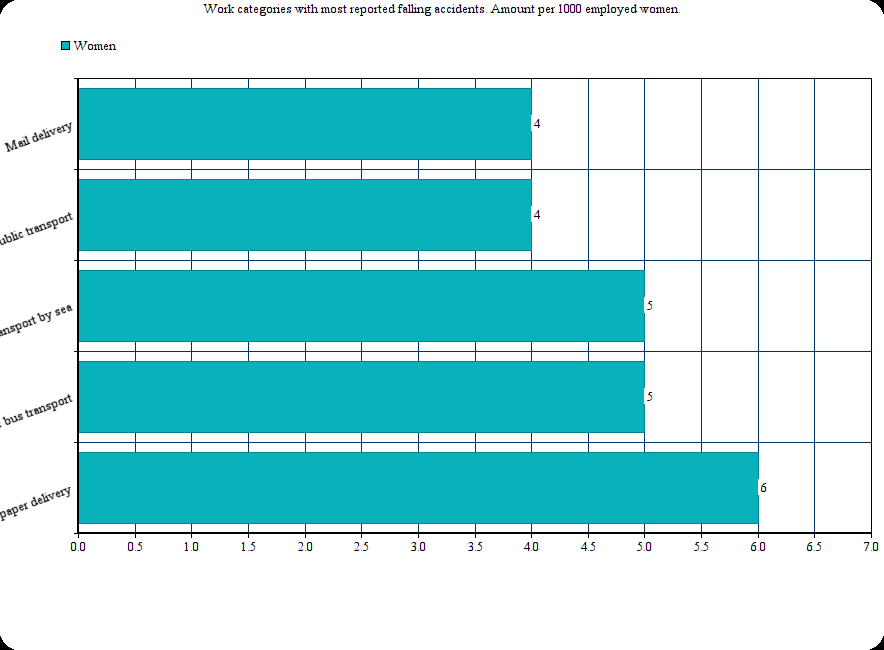
\includegraphics[width=6cm]{../img/Fall_from_ground_women.png} }}%
		\qquad
		\subfloat[label 2]{{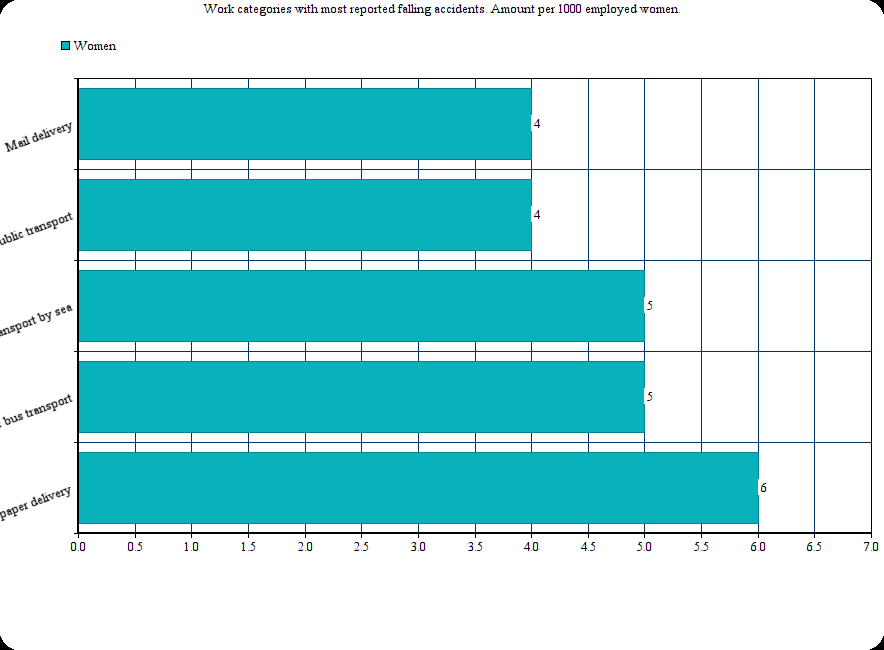
\includegraphics[width=6cm]{../img/Fall_from_ground_women.png} }}%
		\caption{Men and women falling from standing height}%
		\label{fig:example}%
	\end{figure}
	
	\begin{figure}[h]
		\centering
		\subfloat[label 1]{{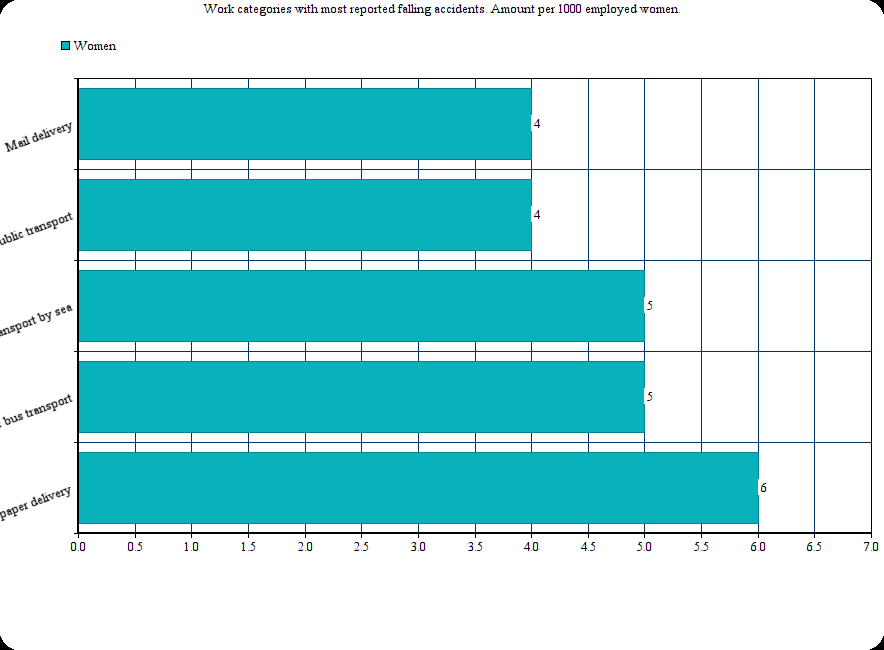
\includegraphics[width=6cm]{../img/Fall_from_ground_women.png} }}%
		\qquad
		\subfloat[label 2]{{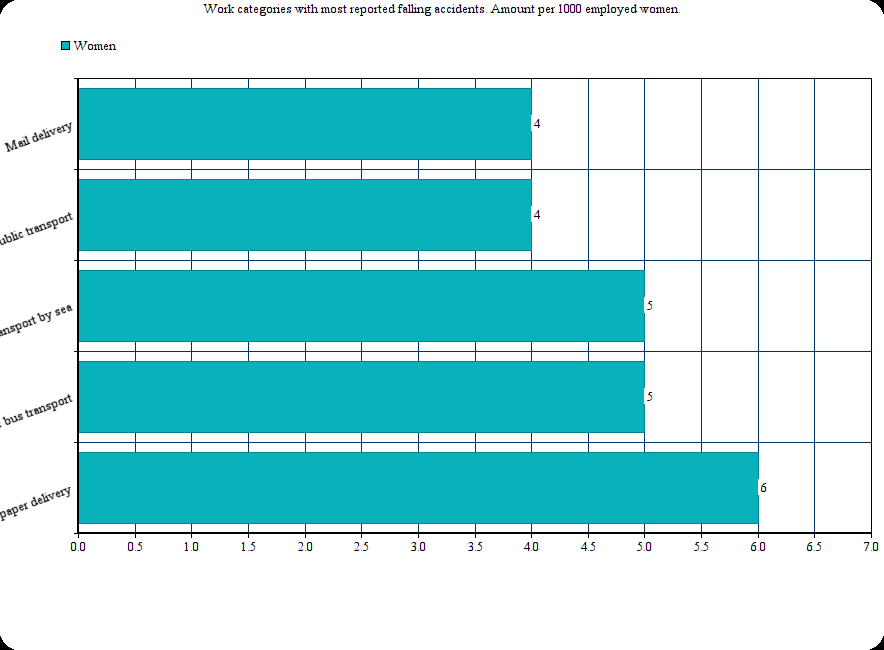
\includegraphics[width=6cm]{../img/Fall_from_ground_women.png} }}%
		\caption{Men and women falling from elevated height}%
		\label{fig:example}%
	\end{figure}
	
	\subsection{Problem}
	
	Falling accidents are common, as described in the background, and it is important that a person who suffers an accident, is aided as quickly as possible to minimize the consequences of the accident. Since a person who suffers a fall may end up in a situation where the person is unable to call for help, for example, because the person is injured or unconscious, an application that could send an automatic alarm could be of great use. An automatic alarm would help minimize the time between the accident and help arriving, since without the alarm, it could take a long time before the person is found by passers-by. For this reason, we want to investigate the possibility of creating a mobile application that can detect falling accidents and report to registered contacts. A mobile application has the advantage that most people already have a smart phone, so if a mobile application could accomplish the task successfully, the cost would be minimized since there will be no need for additional hardware.
	
	This leads us to wonder if it is possible to create such an application, it may be difficult to achieve accuracy in fall detection using only the sensors in the mobile phones that exists on the market today. And if falls were successfully detected, would it be possible to filter out other activities in daily life that resembles falls such as running, jumping or sitting down fast and remain only with the actual falling accidents?
	
	Another question that arises is the fact that this kind of application may have a significant impact on battery life, since it would be necessary to continuously read the sensor values. If the application would drain the battery on the mobile phone, it would make the application far less valuable, since it is unlikely that it would be used.
	
	\subsection{Problem Statement}
	
	This study will aim to answer the questions:
	
	\begin{itemize}
		\item Is it possible to create a mobile application that accurately detects falling accidents using the sensors available in smart phones on the market today?
		\item How will such an application affect the battery life of the mobile phone?
	\end{itemize}
	
	\subsection{Purpose}
	
	The purpose of this thesis is to present the work conducted in the study, and give an answer to the formulated questions.
	
	The purpose of this study is to examine the possibility of creating an application that uses the sensors available in smart phones on the market today to detect falling accidents. This knowledge will be useful for developers interested in creating fall detection software, since it will provide solutions to the problems that we encountered during development. Future developers that want to implement fall detection can use this study to evaluate if the methods used will be right for them.
	
	\subsection{Goal}
	
	The goal of the project is to create an application that, in an effective way, can detect falling accidents and inform concerned contacts. This application should target employees in fields such as operations, construction, etc., and should run in the users cell phone. The user of the application should be able to register contact information to relatives, colleagues, etc. After that the user can activate the protection in the application by selecting the appropriate option, for example by pressing a button in the application. The user is supposed to do this before starting a critical operation such as performing work on an elevated height or similar. When the protection in the application is activated the application makes use of the device's embedded accelerometer to register changes in velocity. If the user would carry the device running the application with the protection actived, while the user would suffer a falling accident, the application would detect this and enter a warning state. In the warning state the application will notify the user that a fall has been detected and that the application soon will send an alarm to registered contacts. If the time limit for the warning state exceeds without any action from the user, an alarm will be sent to the registered contacts using for example SMS.
	
	According to the company that we will work together with, the most important feature is fall detection. It is important that we develop both an Android implementation and an iOS implementation. If we suffer from a lack of time we will not prioritize user interfaces and integration with other functionality, but focus on fall detection. The project will be reported to the company by handing over a GitHub repository.
	
	
	\subsubsection{Sustainability \& Community benefits}
	
	Since the application will not replace any existing technology it is difficult to discuss in which way the application will affect the environment. Our project will be focusing on software alone and will only use hardware that already exists, and thus it will not affect the environment in greater extent. You could however argue that since the application will run on a cell phone, that will draw more current if it runs an additional application in the background, our project will affect the environment but it is hard to say how great such an effect will be.
	
	From a social perspective we hope that the application will contribute to the society in a positive way, since the intention is that the application will help to minimize the negative consequences of accidents related to falling. Hopefully, the finished application will contribute to a better working environment for the users of the application, since an accident may be discovered earlier.  
	
	\subsubsection{Ethics}
	
	One important question when it comes to ethics is how personal data in the application will be handled. The users of the application will need to enter things like password, email address, etc., which should be regarded as sensitive data that must not be viewed by a third party. Besides this, we need to make sure that the application does not have any obvious security vulnerability that makes it possible for a malicious person or organization to acquire the sensitive data in the application.
	
	Another important question is what guarantees the application provides to its users. Since the application is supposed to help users in case of an accident it will be sensitive if the application turns out to function worse than the users expected. The false negative cases, when the user is involved in an accident but the application fails to register this, must be kept to a minimum, but it must also be clear in the description of the application that such cases may occur.
	
	\subsection{Methodologies / Methods}
	
	The first part of the research will be to perform a literature study, where we will gain deeper knowledge in the subject, and find out what earlier attempts have been made to solve this problem. The literature study will give a good starting point for the rest of the study. The next step will be a case study where we develop a mobile application that uses sensors available in smart phones to achieve accurate fall detection. Developing such an application will give us the opportunity to test theories and ideas found in the literature study. Lastly, the applications impact on battery life will be tested by performing experiments using mobile phones running the application.
	
	\subsection{Limitations}
	
	Although there are numerous platforms for mobile applications, we will only consider the two most widely used, Android and iOS.
	
	We believe that there are many fields that could benefit from the type of application that we will develop, but for this study we will only consider implementing it for an electrical company.
	
	\subsection{Disposition}
	
	\newpage
	
	\section{Theoretical Background}
	
	\paragraph{The physics of falling} have been researched on several occasions and the results can be read in a multitude of scientific papers and reports. Much of the research done in this area tries to distinguish the characteristics of a fall in comparison to other motional patterns conducted on a daily basis. For a fall detection system to be considered as reliable it is imperative that it has the means to separate actual fall accidents from other patterns resulting from activities of daily living (further referenced as ADL) to a fair extent. The earth's gravitational pull produces a constant acceleration by 9.8s m/$s^{2}$ towards the ground. This constant acceleration is also referenced as \textit{1g}. A fall would towards the earth's surface would thus initially mean a decrease in acceleration with respect to this natural constant, followed by a rapid acceleration in the other direction as the device (and possibly the person wearing it) hits either the ground or another surface.
	
	
	\paragraph{} Yildirim et. al takes a general approach to describe the character of several motional types \cite{int_journ}. In their research, they measured the response from a LSM330DLC acceleration sensor located in an Android device. Their approach uses a threshold value to indicate whether the acceleration vector exceeds the allowed limit for a crash. The blue, red and green lines corresponds to the acceleration on any of the three perpendicular axis \textit{X}, \textit{Y} and \textit{Z} shown below.
	
	\begin{figure}[h]
		\centering
		\subfloat{{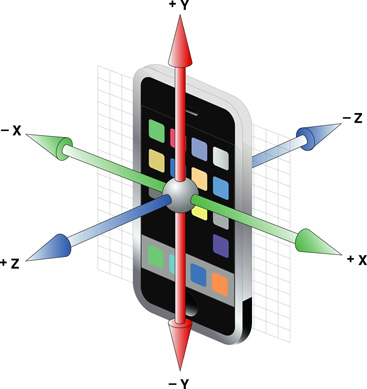
\includegraphics[width=8cm]{../img/accelerometer-axis.jpg} }}%
		\caption{The X, Y and Z axis af a smart phone device}%
		\label{fig:example}% 
	\end{figure}
	
	\begin{figure}[h]
		\centering
		\subfloat{{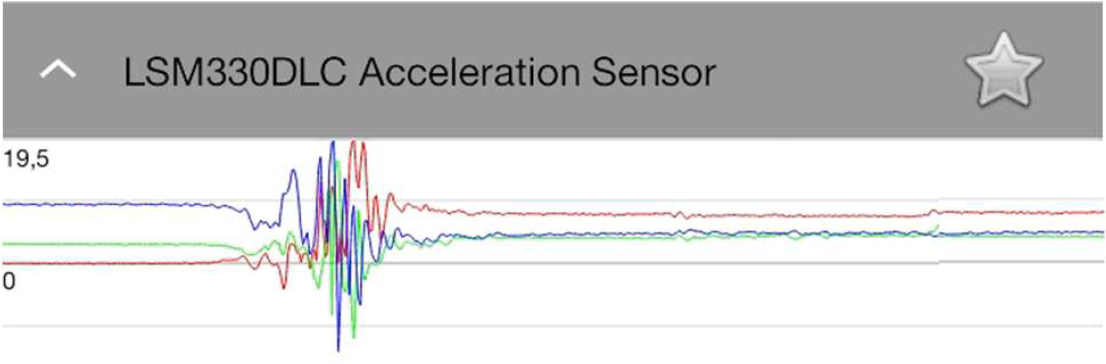
\includegraphics[width=8cm]{../img/Falling.png} }}%
		\caption{The typical pattern of falling}%
		\label{fig:example}%
	\end{figure}
	
	\noindent This measurements shows that falling, as was previously theorized, is indicated by a significant drop in acceleration towards the earth's gravitational pull, signaling that the device is moving towards a free fall state.This drop is then followed by an acceleration spike as the device hits the ground. If a person were to get seriously injured due to a fall s/he would usually remain still on the ground for a period of time. Acceleration would thus gradually go back to the normal \textit{1g} indicated by the flat line after the peak. 
	
	
	\begin{figure}[h]
		\centering
		\subfloat{{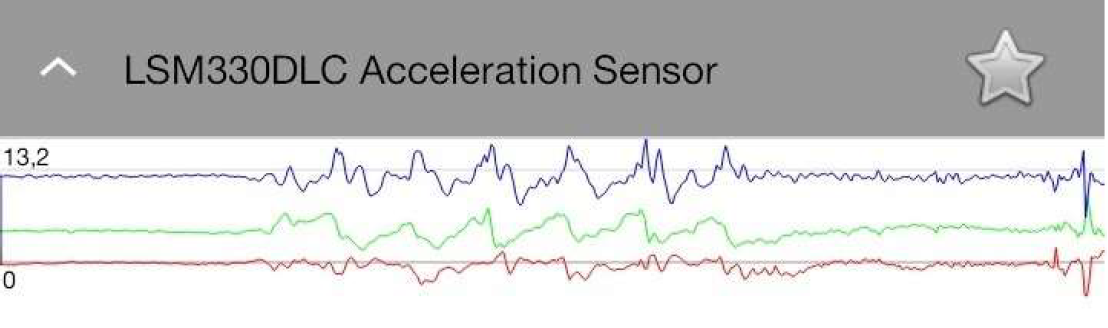
\includegraphics[width=8cm]{../img/Walking.png} }}%
		\caption{The typical pattern of walking}%
		\label{fig:example}%
	\end{figure}
	
	\noindent Walking shows a completely different pattern. As can be seen, the changes in acceleration are not rapid like the previous example. They are also repetitive, meaning that there is no longer period of non-movements after any of the peaks. The peaks them selves are also significant less than in the case of falling shown above. This implies that walking is easily distinguished from falling.
	
	
	
	\begin{figure}[h]
		\centering
		\subfloat{{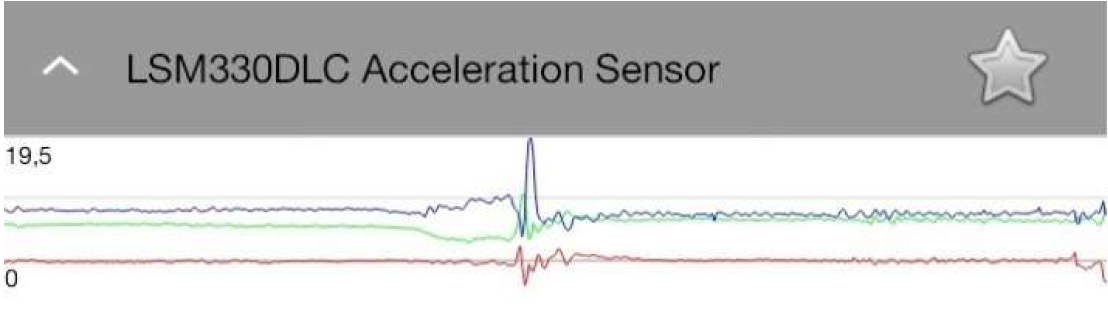
\includegraphics[width=8cm]{../img/Sitting_down.png} }}%
		\caption{The typical pattern of sitting down}%
		\label{fig:example}%
	\end{figure}
	
	\noindent Sitting down on a surface shows a similar pattern to falling with regards to a sudden drop in acceleration followed by  a rapid spike and a longer period of non-movement. The magnitude of these values are however far less than in the case of a fall and should thus be easy to single out. When a person sits down, s/he usually makes a soft movement towards the surface which is matched by the lesser accelerational  magnitude in all three directions \textit{X, Y} and \textit{Z}.
	
	
	\begin{figure}[h]
		\centering
		\subfloat{{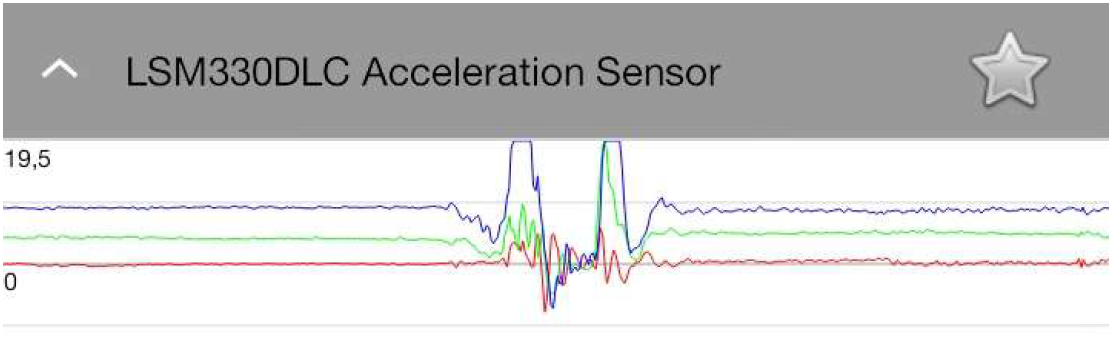
\includegraphics[width=8cm]{../img/Jumping.png} }}%
		\caption{The typical pattern of jumping}%
		\label{fig:example}%
	\end{figure}
	
	\noindent Jumping is according to Yildirim et. al. the hardest pattern to distinguish from a fall. The pattern has a sudden drop in acceleration, followed by a large spike as the jumper crouches and accelerates upwards. After this comes yet another sudden drop in acceleration as the jumper reaches the maximum altitude and starts falling back to earth again. From this part the pattern is almost identical to that of falling. When the jumper falls back to earth, the acceleration drops and then causes another huge spike as s/he hits the ground. When thinking about it, jumping and falling are in fact similar motional types, with the difference that jumping is prefixed by a drop and a spike before becoming an actual fall. The main challenge here is thus to be able to differentiate this from an unintentional falling accident.
	
	
	\paragraph{} Abbatea et. al. takes the above approach further by trying to establish a more sophisticated algorithm that utilizes more than merely just an acceleration vector compared to a threshold value to distinguish a fall like motional pattern from other types of ADL. Their thesis rely on several guidelines which among other include: 
	\begin{itemize} 
		\item "Detection of falls should be carried out using only acceleration-based information. Previous work demonstrated that acceleration is the most reliable information that can be used in detecting a fall, while other kinematic data, such as angular velocity, is less relevant." \cite[p~3]{piza_uni}
		
		\item "Still for usability reasons, the fall detection algorithm should work only with the magnitude of acceleration and not with the values along each of the three accelerometer’s axes, as this, again, would require a known and fixed orientation of the device with respect to the user’s body." \cite[p~3]{piza_uni}
	\end{itemize}
	
	The latter identifies the importance of calculating the resultant vector that comprises the sum of all three vectors \textit{X}, \textit{Y} and \textit{Z}. This vector is the overall acceleration imposed on the device (and possibly the person carrying it). They proceed by defining a \textit{fall-like-event} as "an acceleration greater than \textit{3g} followed by a period of \textit{2500ms} without further peaks exceeding the threshold." \cite[p~5]{piza_uni}. They further argue that the threshold \textit{3g} is chosen since it has been widely used in other types of fall detection systems. According to their experiments, a post-fall event usually means that the body of the unfortunate becomes lying still on the ground after a period of about \textit{1000ms}. This interval, which resides within the \textit{2500ms} interval prior to fall detection is often due to minor peaks following the main impact as a result of that parts of the body/device may hit the ground at different times. 
	
	\paragraph{} Abbatea et. al. tries to establish their algorithm using a \textit{finite-state-machine} with five distinct states.
	
	\begin{itemize}
		\item The \textit{sampling} state is the normal state that the process resides in until \textit{threshold-peak} is detected.
		
		\item When a peak occurs that exceeds the threshold value of \textit{3g} the state is transferred to \textit{post peak}. Well in this state, a bouncing timer of \textit{1000 ms}is started, if another peak exceeding the threshold occurs during this time, bouncing timer is reset, otherwise the state machine moves on to the \textit{post fall} state when the timer fires.
		
		\item In the \textit{post fall state} no peaks exceeding the threshold are allowed during \textit{1500 ms}, or the system goes back to the \textit{post peak} state. The purpose if this state is to check for activity (movement). If another peak occurs, it signals that either is the presumed fall not finished, or the subject is moving and this should not regarded as a fall. 
		
		\item When the \textit{post fall timer} after 1500 ms, the state machine moves on to the \textit{activity test} state. In this test, if movement exceeding certain thresholds are detected, it once again signals that activity is found an that this was indeed not an actual fall but rather a result of ADL. 
		
	\end{itemize}  
	
	\begin{figure}[h]
		\centering
		\subfloat{{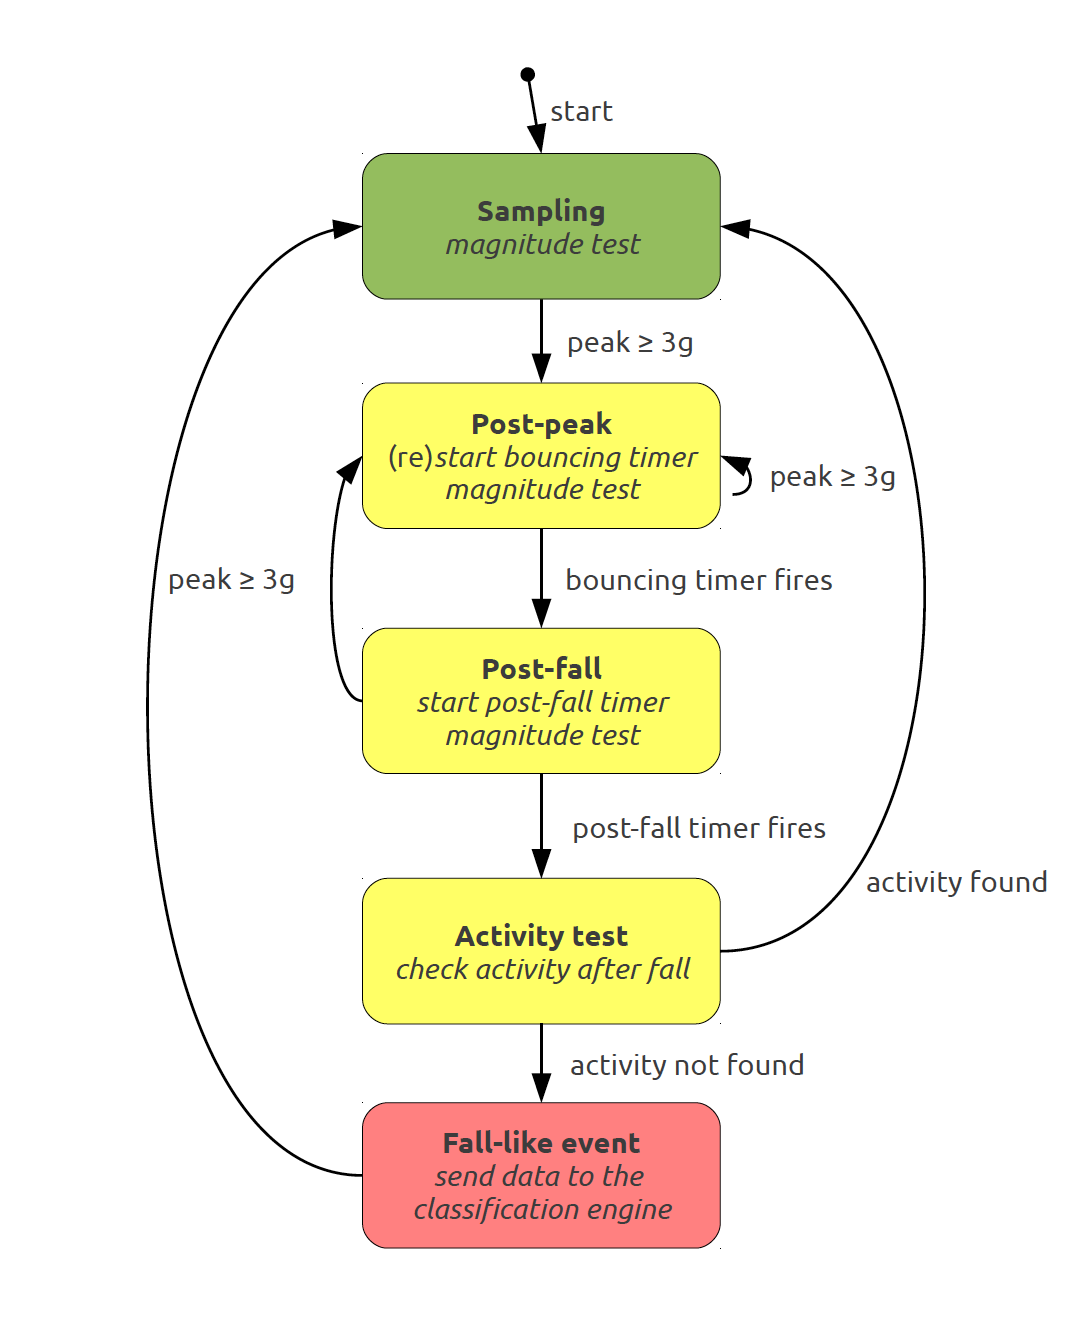
\includegraphics[width=8cm]{../img/Abbatea_finite_state_machine.png}}}%
		\caption{The sensing process discussed in Abbatea et. al.}%
		\label{fig:example}%
	\end{figure}
	
	\paragraph{} if a fall like event has passed through \textit{activity test} (the last state in the state machine), it is fed through a feature extractor, which analyses the data and extract specific and predefined features of the data set which are commonly seen in fall like events. 
	
	\section{Methodologies and Methods}
	
	This chapter describes the research strategy and the methodologies used in the study, and how each methodology will contribute to the research question.
	
	\subsection{Research Strategy}
	
	In order to give an answer to the first question of our problem statement, if it is possible to create a mobile application that accurately detects falling accidents using the sensors available in smart phones on the market today, we need to solve a number of sub problems. The first problem is to find a suitable algorithm that can achieve accurate fall detection, since without a good algorithm it will be impossible to make a useful implementation. The second problem is to implement this algorithm in a mobile application using the sensors available in smart phones. This could be troublesome if the algorithm expects better sensors than what is available in the smart phone. The third sub problem is to evaluate the implementation's impact on battery life. For these sub problems we formulate specific questions that we will need to answer in order to answer the problem statement.
	
	\begin{itemize}
		\item What algorithm should be used to accurately detect a fall?
		\item How can technology available in smart phones be used to implement an algorithm for fall detection?
		\item How can performance issues be minimized when implementing fall detection in a smart phone?
	\end{itemize}
	
	\subsubsection{Research Methods}
	
	This section describes the chosen methodologies, and how they will contribute to solving the problem statement.
	
	\paragraph{Literature Study}
	
	The literature study that we will perform will focus on finding an algorithm that can be used to accurately detect a fall. Performing a literature study will give us a wider understanding of the subject as well as a good starting point for the study. The result of the literature study will show which algorithm for fall detection that would be proposed by earlier studies. We will use this algorithm as a starting point for our own implementation, where we will try to improve the algorithm. The outcome of the literature study is presented in the theoretical background.
	
	\paragraph{Developing a mobile application}
	The second part of our research will be a case study where we implement a fall detection system. We will use the algorithm found in the literature study and implement it for Android and iOS using the sensors available in the smart phones. Developing the application will give us an opportunity to test the algorithm on real devices, and a platform where we can experiment in order to improve the algorithm. The result of the development will give us the ability to answer how technology available in smart phones can be used to implement the algorithm found in the literature study.
	
	\paragraph{Evaluating the implemented mobile application}
	
	The third part of our research will be to evaluate the implemented algorithm by performing experiments where the mobile application is used to detect falls. This evaluation will focus on how accurate the application is, but also on how it affects the battery life of the device.
	
	\subsubsection{Research Process}
	
	In this thesis project, the work is divided in phases. The first phase, the problem statement serves to formulate the problem that the thesis will try to solve. The second phase is the literature study, where reports from earlier studies are collected and read to give us a deeper understanding of the subject. The third phase is the analysis phase, where the results of the literature study is analysed in order to find an algorithm that will be suitable as a starting point for the application. After the analysis phase the case study begins where we will implement the mobile application. After the case study phase the evaluation phase starts, where the final version of the application developed in the case study is evaluated. After that, the conclusion phase starts, where the results are summarized and conclusions formulated. 
	
	\begin{figure}[h]
		\centering
		\subfloat{{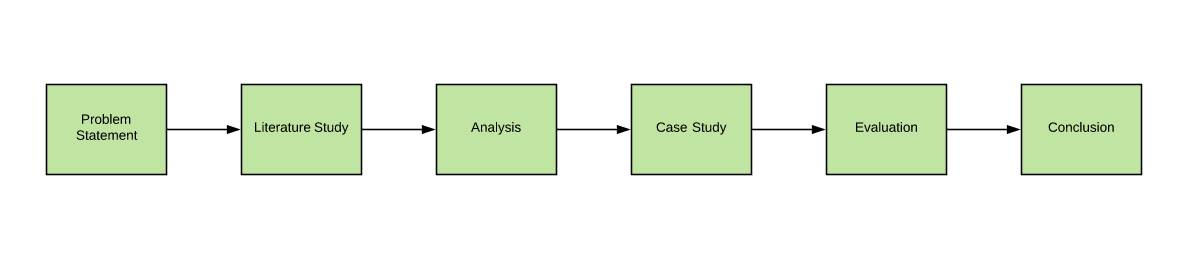
\includegraphics[width=14cm]{../img/method-phases.png} }}%
		\caption{The different phases in the thesis project}%
		\label{fig:example}%
	\end{figure}
	
	\subsection{Design and Implementation of Application}
	
	To develop the mobile application we will use an iterative development method. By using an iterative method we will make sure that the most important features are developed first, since we will develop the most important features in the first iteration and only after that continue with the less important features. This will help us  minimize the risks in the project. If the project would suffer from lack of time, we would at least have developed the most important features already. The project method that we will be using will be similar to Scrum, although since we are only two developers, the team involved in development will be much smaller than the typical agile team.
	
	We will divide the work in such a way that one of us will develop the Android implementation, and one of us will develop the iOS implementation. By dividing the work in this fashion we can implement similar features in both applications without the risk of writing conflicting code. Another reason for dividing the work is that it will help us to have equal focus on both the Android and iOS implementation.
	
	\subsubsection{Development Process}
	
	The development process will follow the outline in figure \ref{fig:development}. The process will start with design, where an initial version of the application is designed, with only a limited set of features. After that we will implement those features, and then evaluate the developed features and the application. After that we will go back to development, and based on the outcome of the development we will either start over, or continue with new features.
	
	\begin{figure}[h]
		\centering
		\subfloat{{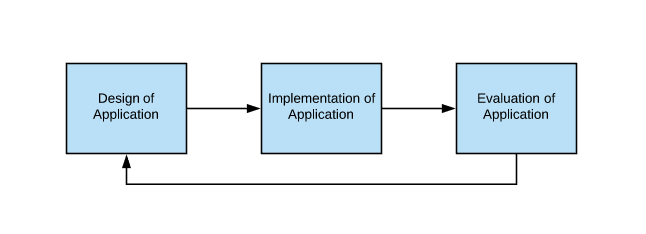
\includegraphics[width=14cm]{../img/method-development.png} }}%
		\caption{The application development process}%
		\label{fig:development}%
	\end{figure}
	
	\subsubsection{Development Environment}
	
	The application will be divided in two implementations, one for Android and one for iOS. The development environment will be slightly different for Android and iOS. 
	
	\paragraph{Android}
	The Android application will be developed using Android Studio, since it is the official development environment.
	
	\paragraph{iOS}
	The iOS application will be partly developed in Xcode, since it is the official IDE, and partly in Jetbrains AppCode since it is superior to Xcode when it comes to re-factoring code, code completion, etc. Xcode will be used for building graphical interfaces, but the coding will be done in AppCode.
	
	\subsection{Evaluation Methods}
	
	This section describes how the developed application will be evaluated. Evaluating the application is important since it will show how well it solves the problem statement.
	
	\subsubsection{Evaluating battery life}
	
	To evaluate how the application affects the battery life of the mobile phone, we will use the native functionality in the operating system available on Android and iOS respectively to measure the specific applications power consumption.
	In combination with this, we will also perform tests where we run the application for a certain amount of time and note how much battery life is left and compare this value with the percentage left after not running the application for the same amount of time.
	
	\subsubsection{Evaluating the fall detection system functionality}
	
	Another step in the evaluation of the application will be to perform crash tests where we measure how well the application detects a fall, by dropping a mobile phone running the application several times from a height that we define as a fall and count the number of reported falls. The same test can then be performed with an existing application to compare how well the implemented algorithm compares to existing technology.
	
	Another measurement will be to drop the mobile phone running the application from a height that we do not define as a fall, and count how many falls are falsely detected. This number will also be compared the result of running the same test with an existing application.
	
	Yet another test will be to perform daily activities that can trigger a fall detection system, even though it is not a fall. Theses activities can be running, or walking with the phone in the pocket. A good fall detection software will not report many of these false positives. This will also be compared against an existing application.
	
	\newpage
	
	\section{Challenges and Possibilites}
	\newpage
	
	\section{Fall Detection Application: Design and Implementation}
	\newpage
	
	\section{Fall Detection Application: Evaluation}
	\newpage
	
	\section{Conclusions}
	\newpage
	
	\bibliography{bib_common}
	\bibliographystyle{ieeetr}
	
\end{document}